\documentclass[border=6pt]{standalone}
\usepackage[T1]{fontenc}
\usepackage{courier}
\usepackage[scaled=0.95]{helvet}
\renewcommand{\familydefault}{\sfdefault}
\usepackage{sfmath}
\usepackage[version=4]{mhchem}
\usepackage{tikz}
\usepackage{pgfplots}
\pgfplotsset{compat=newest}
\usetikzlibrary{arrows.meta,positioning,calc,fit,backgrounds,shapes.geometric,decorations.pathreplacing,patterns}
\definecolor{ink}{HTML}{17233A}
\definecolor{inksoft}{HTML}{44506A}
\definecolor{teal}{HTML}{0E6B6B}
\definecolor{tealsoft}{HTML}{E5F0EF}
\definecolor{amber}{HTML}{B26B12}
\definecolor{ambersoft}{HTML}{FBF0DF}
\definecolor{blue}{HTML}{2F6690}
\definecolor{bluesoft}{HTML}{E3ECF4}
\definecolor{plum}{HTML}{7A4D8C}
\definecolor{plumsoft}{HTML}{EFE7F3}
\definecolor{greyc}{HTML}{8A94A3}
\definecolor{linec}{HTML}{D3DCE1}
\definecolor{oxy}{HTML}{C0392B}
\definecolor{carb}{HTML}{3B4252}
\definecolor{hyd}{HTML}{E6E9EE}
\definecolor{nit}{HTML}{2F6690}
\tikzset{
  every picture/.style={line cap=round,line join=round},
  lab/.style={font=\small, text=inksoft},
  >={Stealth[length=7pt]},
}
\pgfplotsset{
  every axis/.append style={axis line style={inksoft}, tick style={inksoft}, tick label style={font=\footnotesize, text=inksoft}, label style={font=\small, text=ink}},
}
% fragment tile: \frag{node name}{position}{colour}{content}
\newcommand{\frag}[4]{\node[draw=#3, fill=#3!12, line width=1.4pt, rounded corners=6pt, minimum width=1.25cm, minimum height=1.05cm, text=#3, font=\bfseries] (#1) at (#2) {#4};}
\newcommand{\ring}{\tikz[baseline=-0.6ex]{\draw[line width=1.1pt] (0:0.3)--(60:0.3)--(120:0.3)--(180:0.3)--(240:0.3)--(300:0.3)--cycle; \draw[line width=0.8pt] (0,0) circle (0.16);}}
\newcommand{\bond}[2]{\draw[ink, line width=2.2pt] (#1) -- (#2);}

\begin{document}
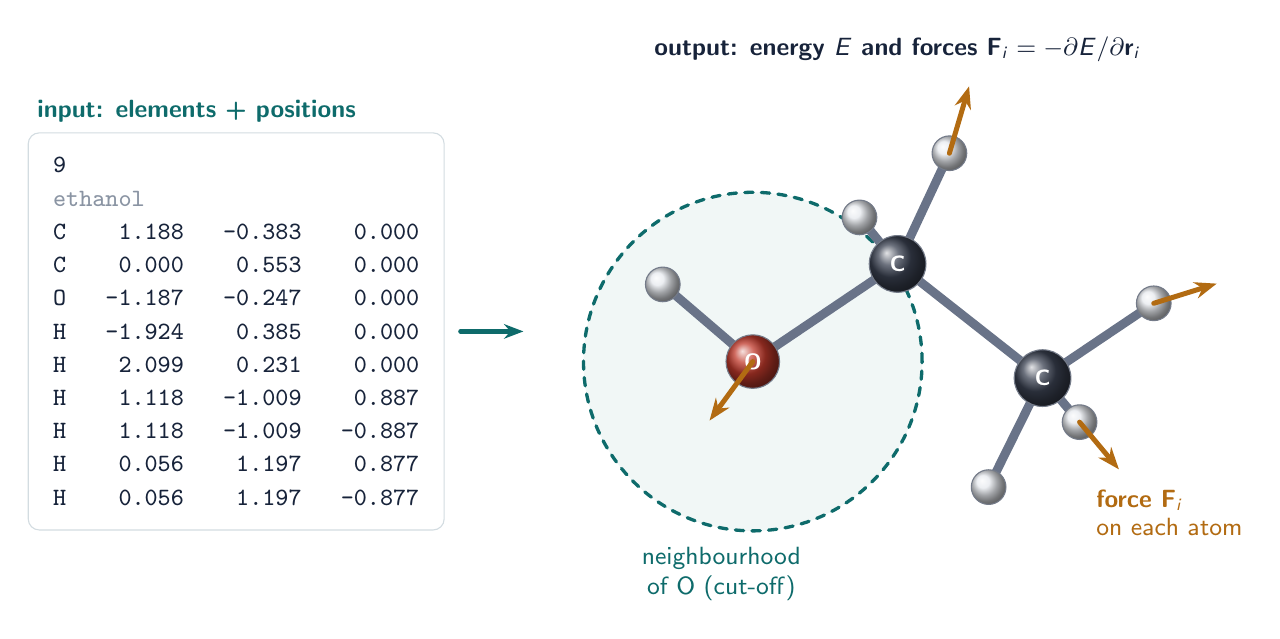
\begin{tikzpicture}
\node[draw=linec, fill=white, rounded corners=4pt, inner sep=9pt, align=left, font=\small, text=ink] (xyz) at (-8.4,0) {\texttt{9}\\[1pt]\texttt{\textcolor{greyc}{ethanol}}\\[1pt]\texttt{C~~~~1.188~~~-0.383~~~~0.000}\\[1pt]\texttt{C~~~~0.000~~~~0.553~~~~0.000}\\[1pt]\texttt{O~~~-1.187~~~-0.247~~~~0.000}\\[1pt]\texttt{H~~~-1.924~~~~0.385~~~~0.000}\\[1pt]\texttt{H~~~~2.099~~~~0.231~~~~0.000}\\[1pt]\texttt{H~~~~1.118~~~-1.009~~~~0.887}\\[1pt]\texttt{H~~~~1.118~~~-1.009~~~-0.887}\\[1pt]\texttt{H~~~~0.056~~~~1.197~~~~0.877}\\[1pt]\texttt{H~~~~0.056~~~~1.197~~~-0.877}};
\node[font=\small\bfseries, text=teal, anchor=south west] at (xyz.north west) {input: elements + positions};
\draw[->, teal, line width=1.6pt] ($(xyz.east)+(0.2,0)$) -- ($(xyz.east)+(1.0,0)$);
\begin{scope}
\draw[teal, dashed, line width=1.2pt, fill=tealsoft, fill opacity=0.55] (-1.839,-0.383) circle (2.15);
\draw[inksoft!80, line width=3.2pt] (1.841,-0.593) -- (0.000,0.857);
\draw[inksoft!80, line width=3.2pt] (0.000,0.857) -- (-1.839,-0.383);
\draw[inksoft!80, line width=3.2pt] (-1.839,-0.383) -- (-2.982,0.597);
\draw[inksoft!80, line width=3.2pt] (1.841,-0.593) -- (3.253,0.357);
\draw[inksoft!80, line width=3.2pt] (1.841,-0.593) -- (2.311,-1.152);
\draw[inksoft!80, line width=3.2pt] (1.841,-0.593) -- (1.156,-1.977);
\draw[inksoft!80, line width=3.2pt] (0.000,0.857) -- (0.658,2.263);
\draw[inksoft!80, line width=3.2pt] (0.000,0.857) -- (-0.484,1.448);
\shade[ball color=hyd, draw=ink!60, line width=0.4pt] (1.156,-1.977) circle (0.22);
\shade[ball color=hyd, draw=ink!60, line width=0.4pt] (-0.484,1.448) circle (0.22);
\shade[ball color=carb, draw=ink!60, line width=0.4pt] (1.841,-0.593) circle (0.36);
\node[font=\footnotesize\bfseries, text=white] at (1.841,-0.593) {C};
\shade[ball color=carb, draw=ink!60, line width=0.4pt] (0.000,0.857) circle (0.36);
\node[font=\footnotesize\bfseries, text=white] at (0.000,0.857) {C};
\shade[ball color=oxy, draw=ink!60, line width=0.4pt] (-1.839,-0.383) circle (0.34);
\node[font=\footnotesize\bfseries, text=white] at (-1.839,-0.383) {O};
\shade[ball color=hyd, draw=ink!60, line width=0.4pt] (-2.982,0.597) circle (0.22);
\shade[ball color=hyd, draw=ink!60, line width=0.4pt] (3.253,0.357) circle (0.22);
\shade[ball color=hyd, draw=ink!60, line width=0.4pt] (0.658,2.263) circle (0.22);
\shade[ball color=hyd, draw=ink!60, line width=0.4pt] (2.311,-1.152) circle (0.22);
\draw[amber, line width=1.8pt, -{Stealth[length=8pt]}] (-1.839,-0.383) -- ++(-0.55,-0.75);
\draw[amber, line width=1.8pt, -{Stealth[length=8pt]}] (3.253,0.357) -- ++(0.80,0.25);
\draw[amber, line width=1.8pt, -{Stealth[length=8pt]}] (0.658,2.263) -- ++(0.25,0.85);
\draw[amber, line width=1.8pt, -{Stealth[length=8pt]}] (2.311,-1.152) -- ++(0.50,-0.60);
\node[font=\small, text=teal, align=center] at (-2.239,-3.083) {neighbourhood\\of O (cut-off)};
\node[font=\small\bfseries, text=amber, align=left, anchor=west] at (2.4,-2.3) {force $\mathbf{F}_i$\\[-1pt]{\mdseries on each atom}};
\end{scope}
\node[font=\small\bfseries, text=ink, anchor=south] at (0,3.3) {output: energy $E$ and forces $\mathbf{F}_i=-\partial E/\partial \mathbf{r}_i$};
\end{tikzpicture}
\end{document}
